
若曾经使用过GNU Make,应该已经了解过目标的概念。本质上,它是构建系统用来将文件列表编译为另一个文件的一个方式。它可以是一个编译成.o对象文件的.cpp实现文件,一组打包成.o静态库的.o文件,以及许多其他组合。

然而,CMake可以节省时间,跳过这些食谱的中间步骤,其可以在更高的抽象级别上工作。CMake会理解如何直接从源文件构建可执行文件。因此,不需要编写显式的配方来编译任何目标文件。所需要的只是一个add\_executable()指令,该指令带有可执行目标的名称和将成为其元素的文件列表:

\begin{lstlisting}[style=styleCMake]
add_executable(app1 a.cpp b.cpp c.cpp)
\end{lstlisting}

我们已经在前面的章节中使用了这个指令,并且已经知道了在实践中如何使用可执行目标——生成步骤中,CMake将创建一个构建系统,并将其填充为方案编译每个源文件,并将它们链接到单个二进制可执行文件中。

在CMake中,可以使用以下指令创建目标:

\begin{itemize}
\item 
add\_executable()

\item 
add\_library()

\item 
add\_custom\_target()
\end{itemize}

前两个不言自明,在前几章中已经简要地使用过它们来构建可执行程序和库(我们将在第5章中深入讨论)。但是这些定制目标是什么呢?

其允许你指定自己的命令行,在不检查输出是否最新的情况下执行,例如:

\begin{itemize}
\item 
计算其他二进制文件的校验和。

\item 
运行代码消毒程序并收集结果。

\item 
向数据处理管道发送编译报告。
\end{itemize}

下面是add\_custom\_target()指令的完整签名:

\begin{lstlisting}[style=styleCMake]
add_custom_target(Name [ALL] [command1 [args1...]]
				[COMMAND command2 [args2...] ...]
				[DEPENDS depend depend depend ... ]
				[BYPRODUCTS [files...]]
				[WORKING_DIRECTORY dir]
				[COMMENT comment]
				[JOB_POOL job_pool]
				[VERBATIM] [USES_TERMINAL]
				[COMMAND_EXPAND_LISTS]
				[SOURCES src1 [src2...]])
\end{lstlisting}

不会在这里详述每个选项,但定制目标不一定要以文件的形式产生工件。

定制目标的一个好的用例,可能是需要在每个构建中删除特定的文件——例如,以确保代码覆盖率报告不包含过时的数据。需要做的就是像这样定义一个自定义目标:

\begin{lstlisting}[style=styleCMake]
add_custom_target(clean_stale_coverage_files
		COMMAND find . -name "*.gcda" -type f -delete)
\end{lstlisting}

上面的命令将搜索所有扩展名为.gcda的文件,并删除它们。不过有一个问题;与可执行目标和库目标不同,自定义目标只有添加到依赖关系图中才会构建。

\subsubsubsection{4.2.1\hspace{0.2cm}依赖图}

成熟的应用通常是由许多组件构建,这里指的不是外部依赖关系。具体来说是内部库。从结构的角度来看,将它们添加到项目中是有用的,可以将相关的东西打包在一个逻辑实体中,还可以链接到其他目标——另一个库或可执行文件。当多个目标使用同一个库时,这尤其方便。请看图4.1,其描述了一个示例依赖性图:

\begin{center}
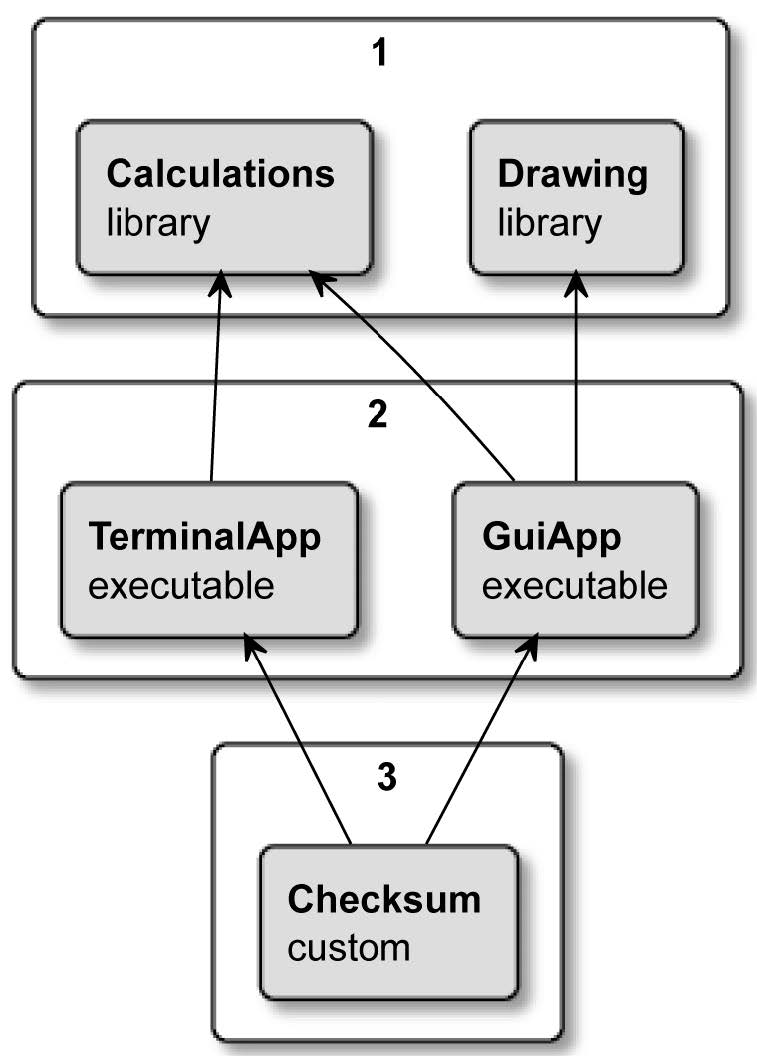
\includegraphics[width=0.4\textwidth]{content/2/chapter4/images/1.jpg}\\
图4.1  BankApp项目中构建依赖的顺序
\end{center}

这个项目中,有两个库、两个可执行程序和一个自定义目标。这里的用例是为用户提供一个银行应用,该应用程序具有一个漂亮的GUI(GuiApp),以及一个命令行版本,可作为自动化脚本(TerminalApp)的一部分使用。两个可执行程序都依赖于相同的计算库,但只有一个需要绘图库。为了确保应用程序下载正确,将计算一个校验和,将其存储在一个文件中,并通过单独的安全通道分发它。CMake在为这样的解决方案编写列表文件时非常灵活:

\begin{lstlisting}[style=styleCMake]
# chapter04/01-targets/CMakeLists.txt

cmake_minimum_required(VERSION 3.19.2)
project(BankApp CXX)

add_executable(terminal_app terminal_app.cpp)
add_executable(gui_app gui_app.cpp)

target_link_libraries(terminal_app calculations)
target_link_libraries(gui_app calculations drawing)

add_library(calculations calculations.cpp)
add_library(drawing drawing.cpp)

add_custom_target(checksum ALL
	COMMAND sh -c "cksum terminal_app>terminal.ck"
	COMMAND sh -c "cksum gui_app>gui.ck"
	BYPRODUCTS terminal.ck gui.ck
	COMMENT "Checking the sums..."
)
\end{lstlisting}

使用target\_link\_libraries()指令将库与可执行文件连接起来。若没有它,可执行文件的编译将会因为未定义的符号而失败。我们在实际声明库之前调用了这个命令。当CMake配置项目时,其会收集关于目标,及其属性的信息——名称、依赖项、源文件和其他信息。

解析所有文件之后,CMake将尝试构建一个依赖图。和所有有效的依赖图一样,它们是有向无环图。有着一个明确的方向,确定哪个目标依赖于哪个目标,不过这样的依赖不能形成环。

当在构建模式下执行cmake时,生成的构建系统将检查已经定义的顶级目标并递归构建它们的依赖项。考虑一下图4.1中的例子:

\begin{enumerate}
\item 
从顶部开始,构建第1组中的两个库。

\item 
计算和绘图库完成后,构建组2 - GuiApp和TerminalApp。

\item 
构建一个校验和目标,运行指定的命令行生成校验和(cksum是一个Unix校验和工具)。
\end{enumerate}

有一个小问题——前面的解决方案并不能保证在可执行文件之后构建校验和目标。CMake不知道校验和依赖于当前的可执行二进制文件,所以可以自由地开始构建。为了解决这个问题,可以把add\_dependencies()指令放在文件的末尾:

\begin{lstlisting}[style=styleCMake]
add_dependencies(checksum terminal_app gui_app)
\end{lstlisting}

这将确保CMake理解Checksum目标和可执行程序之间的关系。

不过target\_link\_libraries()和add\_dependencies()之间有什么区别呢?第一个用于与实际库一起使用,并允许控制属性传播。第二种方法只能用于顶层目标,以设置它们的构建顺序。

随着项目变得越来越复杂,依赖树变得越来越难以理解。如何简化这个过程?

\subsubsubsection{4.2.2\hspace{0.2cm}可视化的依赖性}

即使是小项目也很有难和与其他开发人员直接分享。最简单的方法是通过一个漂亮的图表。毕竟,一张图片胜过千言万语。我们可以自己做这个工作并画一个图表,就像图4.1中所做的那样。但这很没意思,而且需要不断更新。幸运的是,CMake有一个很好的模块来生成点/graphviz格式的依赖关系图。它支持内部和外部依赖关系!

要使用它,可以简单地执行以下命令:

\begin{tcblisting}{commandshell={}}
cmake --graphviz=test.dot .
\end{tcblisting}

该模块将生成一个文本文件,可以将该文本文件导入Graphviz可视化软件,该软件可以渲染图像或生成PDF或SVG文件,这些文件可以作为软件文档的一部分存储。每个人都喜欢好的文档,但是几乎没有人喜欢创建文档——现在,不需要自己来做了!

若赶时间,甚至可以直接从浏览器运行Graphviz,地址如下:

\url{https://dreampuf.github.io/GraphvizOnline/}

\begin{tcolorbox}[colback=blue!5!white,colframe=blue!75!black,title=重要的Note]
自定义目标在默认情况下是不可见的,需要创建一个特殊的配置文件CMakeGraphVizOptions.cmake,可以自定义图形。设置了一个方便的定制命令(GRAPHVIZ\_CUSTOM\_TARGETS TRUE);将其添加到特殊的配置文件中,以支持报告图中的自定义目标。可以在该模块的文档中找到更多选项。
\end{tcolorbox}

所需要做的就是复制和粘贴测试的内容。点文件到左边的窗口,项目将会可视化。很方便,不是吗?

\begin{center}
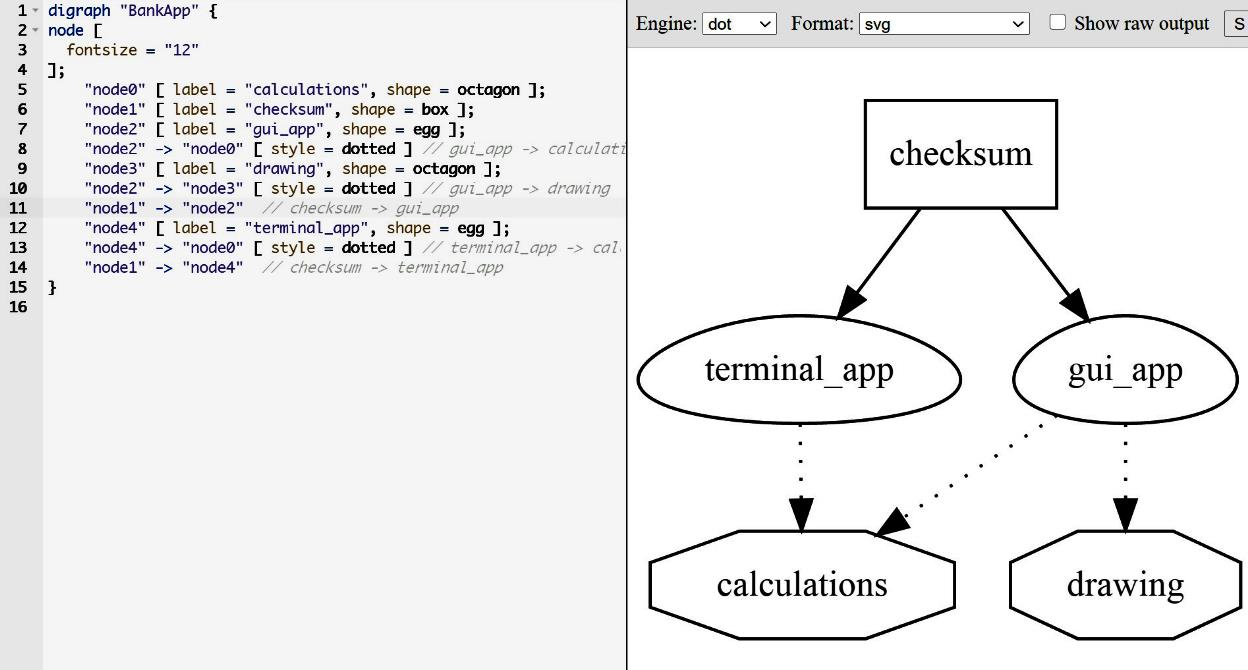
\includegraphics[width=0.8\textwidth]{content/2/chapter4/images/2.jpg}\\
图4.2  Graphviz中BankApp示例的可视化
\end{center}

为了清晰起见,从上图中删除了自动生成的图例部分。

使用这种方法,可以快速地看到所有显式定义的目标。现在有了这个全局视角,让我们深入研究一下如何配置。
 
\subsubsubsection{4.2.3\hspace{0.2cm}目标属性}

目标具有类似于C++对象字段的工作方式的属性。可以修改其中一些属性,而其他属性只读。CMake定义了一个很大的“已知属性”列表(参见扩展阅读部分),这些属性取决于目标的类型(可执行、库或自定义),还可以添加自己的属性。使用以下命令操作目标器的属性:

\begin{lstlisting}[style=styleCMake]
get_target_property(<var> <target> <property-name>)
set_target_properties(<target1> <target2> ...
						PROPERTIES <prop1-name> <value1>
						<prop2-name> <value2> ...)
\end{lstlisting}

要在屏幕上打印目标属性,需要将其存储在<var>变量中,然后message()将其发送给用户,需要一个个地读取。另外面,在目标上设置属性可以在多个目标上同时指定多个属性。

属性的概念并非目标所独有。CMake还支持设置其他作用域的属性:GLOBAL、DIRECTORY、SOURCE、INSTALL、TEST和CACHE。

要操作所有类型的属性,有get\_property()和set\_property()指令。可以使用这些低层指令来做set\_target\_properties()指令所做的事情:

\begin{lstlisting}[style=styleCMake]
set_property(TARGET <target> PROPERTY <name> <value>)
\end{lstlisting}

最好尽可能多地使用高级命令。CMake提供了更多这样的功能,范围甚至更窄,比如在目标上设置特定的属性。例如,add\_dependencies(<target> <dep>)将依赖项附加到MANUALLY\_ADDED\_DEPENDENCIES目标属性中。可以使用get\_target\_property()查询,就像使用其他属性一样。然而,不能使用set\_target\_property()来更改(只读),CMake中使用add\_dependencies()指令只能进行追加操作。

接下来的章节中讨论编译和链接时,将介绍更多的属性设置命令。同时,我们会了解到一个目标的属性如何转换到另一个目标。

\subsubsubsection{4.2.4\hspace{0.2cm}可传递需求}

命名真的很难,有时会得到一个很难理解的结果。不幸的是,“传递性使用需求”是CMake文档中的神秘的主题之一。让我们来了解一下这个奇怪的名字,也许可以想出一个更容易理解的术语。

我将从解释这个谜题的中间部分开始,一个目标可能依赖于另一个目标。CMake文档有时将这种依赖关系称为“使用”,例如在一个目标中使用另一个目标。这个很简单,我们继续下一个。

某些情况下,这样的已用目标具有使用目标必须满足的特定需求:链接一些库,包含一个目录,或要求特定的编译特性。这些实际上都是需求,因此文档在某种意义上是正确的。问题是在文档的其他上下文中都不称其为需求。当为单个目标指定相同的需求时,可以设置属性或依赖项。因此,名称的最后一部分可能应该简单地称为“属性”。

最后一部分是传递,我相信这一点是正确的(也许有点太聪明了)。CMake将使用目标的一些属性/需求附加到使用它们的目标的属性中。可以说某些属性可以隐式地跨目标转换(或简单地传播),因此更容易表示依赖关系。

简化整个概念,将其视为源目标(使用的目标)和目标目标(使用其他目标的目标)之间的传播属性。

来看一个具体的例子,来理解其为什么会存在,以及如何工作的:

\begin{lstlisting}[style=styleCMake]
target_compile_definitions(<source> <INTERFACE|PUBLIC|PRIVATE> 
	[items1...])
\end{lstlisting}

这个目标命令将填充<source>目标的COMPILE\_DEFINITIONS属性。编译定义只是传递给配置C++预处理器定义的编译器的-Dname=定义标志(我们将在第5章中讨论)。有趣的是第二个论点,需要指定三个值INTERFACE、PUBLIC或PRIVATE中的一个,以控制应该将属性传递给哪个目标。现在,不要将这些与C++访问说明符混淆。

传递关键字的工作原理如下:

\begin{itemize}
\item 
PRIVATE设置源目标的属性。

\item 
INTERFACE设置相关目标的属性。

\item 
PUBLIC设置源和相关目标的属性。
\end{itemize}

当不将属性传递到其他目标时,可以将其设置为PRIVATE。

当需要这样的传递时,使用PUBLIC。若源目标在其实现(.cpp文件)中不使用该属性,而只在头文件中使用该属性,这些属性会传递给消费者目标,那么就使用INTERFACE。

这些是如何工作的?为了管理这些属性,CMake提供了一些指令,比如前面提到的target\_compile\_definitions()。当指定PRIVATE或PUBLIC关键字时,CMake将在与指令匹配的目标的属性中存储提供的值——本例中是COMPILE\_DEFINITIONS。此外,若关键字是INTERFACE或PUBLIC,将用INTERFACE\_前缀——INTERFACE\_COMPILE\_DEFINITIONS将值存储在属性中。在配置阶段,CMake将读取源目标的接口属性,并将其内容附加到目标目标。就传播属性,或传递了使用需求。

在CMake 3.20中,可以使用target\_link\_options()或直接使用set\_target\_properties()指令管理12个这样的属性:

\begin{itemize}
\item 
AUTOUIC\_OPTIONS

\item 
COMPILE\_DEFINITIONS

\item 
COMPILE\_FEATURES

\item 
COMPILE\_OPTIONS

\item 
INCLUDE\_DIRECTORIES

\item 
LINK\_DEPENDS

\item 
LINK\_DIRECTORIES

\item 
LINK\_LIBRARIES

\item 
LINK\_OPTIONS

\item 
POSITION\_INDEPENDENT\_CODE

\item 
PRECOMPILE\_HEADERS

\item 
SOURCES
\end{itemize}

我们将在下面的页面中讨论这些选项中,但这些选项都在CMake手册中进行了描述。可以在URL下找到它们的页面(可以用感兴趣的属性替换<PROPERTY>):

\url{https://cmake.org/cmake/help/latest/prop_tgt/<PROPERTY>.html}

下一个问题是这种传播能有多远。属性是在第一个目标上设置的,还是发送到依赖关系图的最顶端?实际上,由使用者来决定。

要在目标之间创建依赖关系,可以使用target\_link\_libraries()指令。此指令的完整签名有一个propagation关键字:

\begin{lstlisting}[style=styleCMake]
target_link_libraries(<target>
					<PRIVATE|PUBLIC|INTERFACE> <item>...
					[<PRIVATE|PUBLIC|INTERFACE> <item>...]...)
\end{lstlisting}

此签名还指定了传播关键字,但此签名控制源目标的属性存储在目标目标中的何处。图4.3显示了在生成阶段(配置阶段完成后)传播属性的变化:

\begin{center}
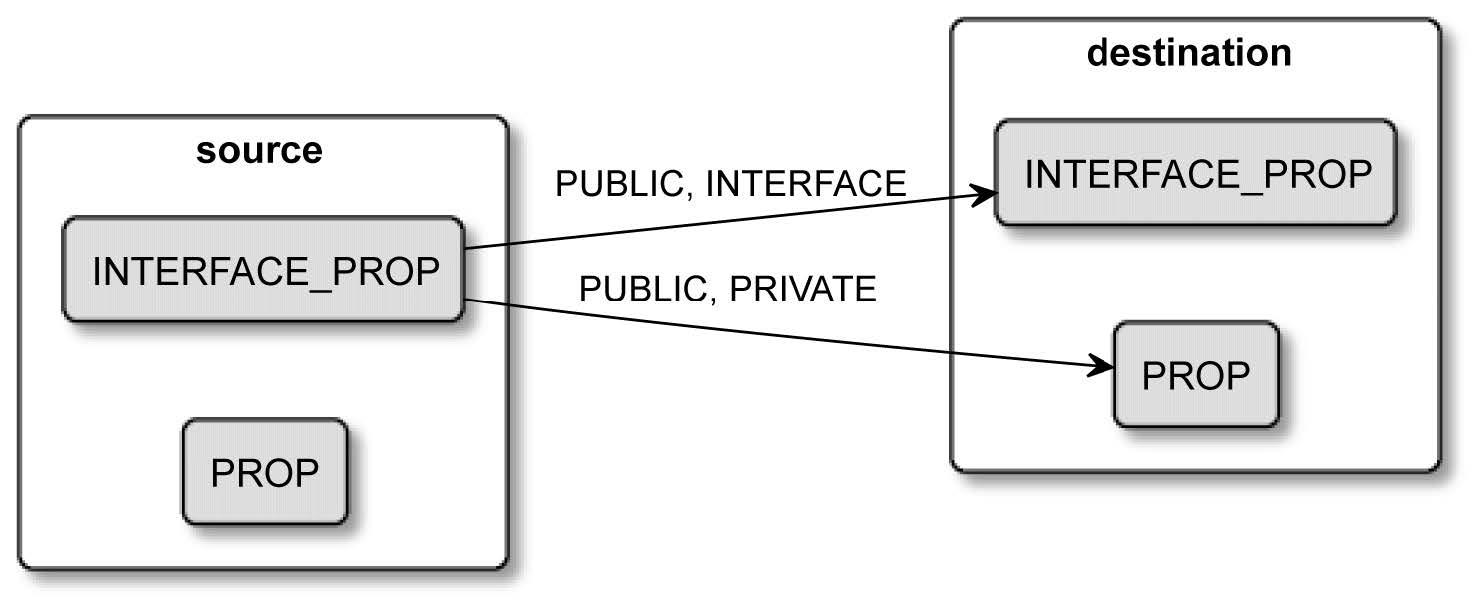
\includegraphics[width=0.8\textwidth]{content/2/chapter4/images/3.jpg}\\
图4.3 属性如何传播到目标
\end{center}

propagation(传播)关键字的工作原理如下:

\begin{itemize}
\item 
PRIVATE将源附加到目标的私有属性。

\item 
INTERFACE将源附加到目标的接口属性。

\item 
PUBLIC包括以上两种属性的特点。
\end{itemize}

接口属性仅用于在链中进一步传播属性,而目标不会在其构建过程中使用它们。

之前使用的基本target\_link\_libraries(<target> <item>…)指令隐式指定PUBLIC关键字。

若正确地为源目标设置了propagation(传播)关键字,属性将自动传递到目的目标上——除非有冲突……

\subsubsubsection{4.2.5\hspace{0.2cm}处理冲突的传播属性}

当目标依赖于多个其他目标时,可能会出现传播属性彼此完全冲突的情况。假设一个使用的目标指定POSITION\_INDEPENDENT\_CODE属性为True,另一个为False。CMake将此理解为冲突,并输出类似如下的错误:

\begin{tcblisting}{commandshell={}}
CMake Error: The INTERFACE_POSITION_INDEPENDENT_CODE property
of "source_target2" does not agree with the value of POSITION_
INDEPENDENT_CODE already determined for "destination_target".
\end{tcblisting}

接收这样的消息很有用,因为明确地知道引入了这个冲突,并且需要解决它。CMake有它自己的属性,这些属性必须在源目标和目标目标之间“一致”。

极少数情况下,这可能会变得很重要——例如,若在多个目标中使用相同的库构建软件,然后链接到单个可执行文件。若这些源目标使用同一个库的不同版本,可能会遇到问题。

为了确保只使用相同的特定版本,可以创建一个自定义接口属性INTERFACE\_LIB\_VERSION,并将版本存储在那里。这还不足以解决问题,因为CMake在默认情况下不会传播自定义属性,必须显式地将自定义属性添加到“兼容”属性列表中。

每个目标都有4个这样的列表:

\begin{itemize}
\item 
COMPATIBLE\_INTERFACE\_BOOL

\item 
COMPATIBLE\_INTERFACE\_STRING

\item 
COMPATIBLE\_INTERFACE\_NUMBER\_MAX

\item 
COMPATIBLE\_INTERFACE\_NUMBER\_MIN
\end{itemize}

将属性附加到其中一个,将触发传播和兼容性检查。BOOL列表将检查传播到目标目标的所有属性是否计算为相同的布尔值。类似地,STRING将求值为字符串。NUMBER\_MAX和NUMBER\_MIN有点不同——传播值不需要匹配,但目标只会接收最高或最低的值。

这个例子将帮助我们理解如何在实践中应用:

\begin{lstlisting}[style=styleCMake]
# chapter04/02-propagated/CMakeLists.txt

cmake_minimum_required(VERSION 3.20.0)
project(PropagatedProperties CXX)

add_library(source1 empty.cpp)
set_property(TARGET source1 PROPERTY INTERFACE_LIB_VERSION
	4)
set_property(TARGET source1 APPEND PROPERTY
	COMPATIBLE_INTERFACE_STRING LIB_VERSION
)
add_library(source2 empty.cpp)

set_property(TARGET source2 PROPERTY INTERFACE_LIB_VERSION
	4)
add_library(destination empty.cpp)
target_link_libraries(destination source1 source2)
\end{lstlisting}

这里创建了三个目标,所有文件都使用相同的空源文件。两个源目标上,用INTERFACE\_前缀指定自定义属性。将它们设置为相同的匹配库版本。两个源目标都链接到目标目标。最后,指定一个STRING兼容性要求作为source1的属性(没有在这里添加INTERFACE\_前缀)。

CMake将这个自定义属性传播到目标目标,并检查所有源目标的版本是否完全匹配(compatibility属性可以只在一个目标上设置)。

既然了解了目标是什么,就看看其他看起来像目标,闻起来像目标,有时也像目标(鸭子定律)。但事实证明,其并不是真正的目标。

\subsubsubsection{4.2.6\hspace{0.2cm}实现伪目标}

目标的概念非常有用,若其一些行为可以借鉴,那就太好了。具体来说,这是指不表示构建系统的输出而是表示输入的东西——外部依赖项、别名等。这些是伪目标,或者没有到达生成的构建系统的目标。

\hspace*{\fill} \\ %插入空行
\noindent
\textbf{导入目标}

若浏览了目录,就会知道将讨论CMake如何管理外部依赖项——其他项目、库等。导入的目标基本上是这个过程的产物。CMake可以定义它们作为find\_ package()指令的结果。

可以调整这样一个目标的目标属性:编译定义、编译选项、包含目录等——甚至将支持可传递的使用需求。但应该将它们视为不可变的,不要改变它们的来源或依赖关系。

导入目标的范围可以是全局的,也可以是本地目录(在子目录中可见,但在父目录中不可见)。

\hspace*{\fill} \\ %插入空行
\noindent
\textbf{别名目标}

别名目标完全符合期望——不同的名称下创建对目标的另一个引用。可以使用以下指令为可执行文件和库创建别名目标:

\begin{lstlisting}[style=styleCMake]
add_executable(<name> ALIAS <target>)
add_library(<name> ALIAS <target>)
\end{lstlisting}

别名目标的属性只读,并且不能安装或导出别名(在生成的构建系统中不可见)。

那么,使用别名的理由到底是什么呢?当项目的某些部分(如子目录)需要具有特定名称的目标时,就很方便了,而实际的实现可能根据情况在不同的名称下可用。例如,可能希望构建一个随解决方案一起提供的库,或者根据用户的选择导入。

\hspace*{\fill} \\ %插入空行
\noindent
\textbf{接口库}

这是一个有趣的构造——一个库不编译任何东西,而是作为一个实用工具目标。其整个概念是围绕传播属性(传递使用需求)构建的。

接口库有两个主要用途——纯头文件库和将一堆传播的属性捆绑到一个逻辑单元中。

使用add\_library(INTERFACE)创建纯头文件库相当容易:

\begin{lstlisting}[style=styleCMake]
add_library(Eigen INTERFACE
	src/eigen.h src/vector.h src/matrix.h
)
target_include_directories(Eigen INTERFACE
	$<BUILD_INTERFACE:${CMAKE_CURRENT_SOURCE_DIR}/src>
	$<INSTALL_INTERFACE:include/Eigen>
)
\end{lstlisting}

前面的代码片段中,创建了一个具有三个头文件的特征接口库。接下来,使用生成器表达式,在导出目标时将其include目录设置为\$\{CMAKE\_CURRENT\_SOURCE\_DIR\}/src,在安装目标时设置为include/Eigen。

要使用这样的库,只需要链接即可:

\begin{lstlisting}[style=styleCMake]
target_link_libraries(executable Eigen)
\end{lstlisting}

这里没有实际的链接,但是CMake将此命令理解为将所有INTERFACE属性传播到可执行目标的请求。

第二个用例使用了完全相同的机制,但目的不同——其创建了一个逻辑目标,可以作为传播属性的占位符。然后,可以将这个目标用作其他目标的依赖项,并以一种简洁、方便的方式设置属性。这里有一个例子:

\begin{lstlisting}[style=styleCMake]
add_library(warning_props INTERFACE)
target_compile_options(warning_props INTERFACE
	-Wall -Wextra -Wpedantic
)
target_link_libraries(executable warning_props)
\end{lstlisting}

add\_library(INTERFACE)指令创建一个逻辑warning\_props目标,用于在可执行目标上设置第二个命令中指定的编译选项。推荐使用这些INTERFACE目标,这提高了代码的可读性和可重用性。可以把它看作是将一堆神奇的值重构为一个命名良好的变量,还建议使用\_props后缀将接口库与常规库区分开来。

伪目标是否耗尽了目标的概念?当然不是!我们仍然需要理解,如何将这些目标转化为生成的构建系统。

\subsubsubsection{4.2.7\hspace{0.2cm}构建目标}

目标这个词有点夸张,在项目的上下文中和生成的构建系统的上下文中意味着不同的东西。当CMake生成一个构建系统时,会将CMake语言中的列表文件“编译”为所选构建工具的语言,也许为GNU Make创建了一个Makefile。这样的Makefile有它们自己的目标——其中一些是列表文件目标的直接转换,另一些是隐式创建的。

这样的构建系统目标是ALL,CMake在默认情况下生成它来包含所有顶层列表文件目标,比如可执行文件和库(不一定是自定义目标)。ALL是在运行cmake -{}-build <build tree>而不选择具体目标时生成的,可以通过向前面的命令添加-{}-target <name>参数来选择一个。

有些可执行程序或库可能不是在每个构建中都需要,但希望将它们作为项目的一部分,以便在有用的时候使用。为了优化默认构建,可以像这样从ALL目标中排除它们:

\begin{lstlisting}[style=styleCMake]
add_executable(<name> EXCLUDE_FROM_ALL [<source>...])
add_library(<name> EXCLUDE_FROM_ALL [<source>...])
\end{lstlisting}

自定义目标则相反——默认情况下,排除在ALL目标之外,除非使用ALL关键字显式地定义它们,就像BankApp示例中那样。

另一个隐式定义的构建目标是干净的,只是从构建树中删除所生成的工件。用它来清除所有旧文件,从头开始构建一切。重要的是要理解它并不是简单地删除构建目录中的所有内容。所以要使clean正确工作,需要手动指定自定义目标可能创建为副产品的文件(请参阅BankApp示例)。

还有一种有趣的非目标机制可以创建可在所有实际目标中使用的自定义工件——自定义命令。

